\section{Our Approach}
As stated earlier, we used compartmental population models to quantify the propagation of news and rumors on Twitter, focusing primarily on the SIS and SEIZ models.

\subsection{SIS}
As described earlier, this model divides the population into two compartments, or classes: susceptible and infected.
Note that in this model, infected individuals return to the susceptible class on recovery because the disease confers no immunity against reinfection.


In order to adapt this model for Twitter, we have given new meaning to these terms. An individual is identified as infected (I) if he posts a tweet about the topic of interest, and susceptible (S) if he has not. A consequence of this interpretation is that an individual posting a tweet is retained to the infected compartment indefinitely; hence, he can not propagate back to the susceptible class as is possible in an epidemiological application. At any given time period $t$, we use $N(t)$ to denote the total population size, $S(t)$ the susceptible population size, and $I(t)$ the infected population size, such that $N(t) = I(t) + S(t)$. As shown in Figure~\ref{fig:sis-framework}, the SIS spreading rule can be summarized as follows:

\begin{figure}[ht]
\centering
%\epsfig{file=word.pdf, width=3in}
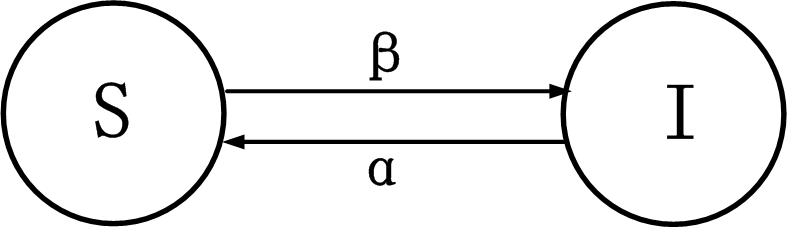
\includegraphics[width=2.5in]{pictures/SIS.png} %?????????????
\vspace{-1em}
\caption{SIS model framework}
\label{fig:sis-framework}
\end{figure}


\begin{figure}[ht]
\centering
%\epsfig{file=word.pdf, width=3in}
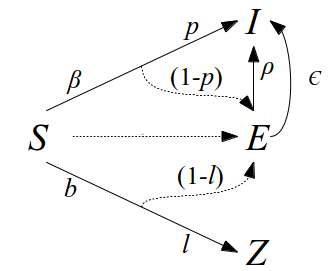
\includegraphics[width=2.5in]{pictures/SEIZ.png} %?????????????
\vspace{-1em}
\caption{SEIZ model framework}
\label{fig:seiz-framework}
\end{figure}


\begin{itemize}
\item An individual that tweets about a topic is regarded as infected.
\item A susceptible person has not tweeted about the topic.
\item A susceptible person coming into contact with an infected individual (via a tweet) becomes infected himself, thus immediately posting a tweet.
\item Susceptible individuals remain so until coming into contact with an infected person.
\end{itemize}

\begin{figure}[t]
\centering
  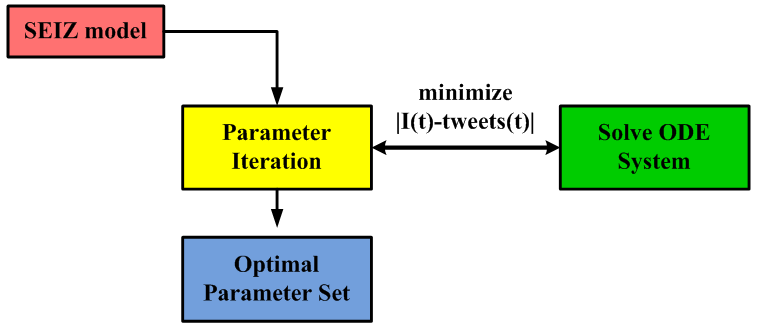
\includegraphics[width=3in]{pictures/implementation_flow.png}
  \vspace{-1em}
  \caption{Numerical implementation work-flow.
 % For both the SIS and SEIZ models, a nonlinear least squares fit of each ODE system to Twitter data identifies an optimal parameter set by minimizing the difference between the Infected compartment and the Twitter data.
  }
  \label{fig:implementation_flow}
\end{figure}

\noindent
The SIS model is mathematically represented by the following system of ordinary differential equations (ODEs)~\cite{murray2002mathematical}:

\begin{subequations}\label{eq:sis}
\begin{align}
&\frac{d [S]}{dt} = -\beta S I + \alpha I \\
&\frac{d [I]}{dt} = \beta S I - \alpha I
\end{align}
\end{subequations}


\subsection{SEIZ}
One drawback of the SIS model is that once a susceptible individual gets exposed to disease, he can only directly transition to infected status. In fact, especially on Twitter, this assumption does not work well; people's ideologies are complex and when they are exposed to news or rumors, they may hold different views, take time to adopt an idea, or even be skeptical to some facts. In this situation, they might be persuaded to propagate a story, or commence only after careful consideration themselves. Additionally, it is quite conceivable that an individual can be exposed to a story (i.e. received a tweet), yet never post a tweet themselves.

Based on this reasoning, we considered a more applicable, robust model, the SEIZ model which was first used to study the adoption of Feynman diagrams~\cite{powerofgoodidea:2006}. In the context of Twitter, the different compartments of the SEIZ model can be viewed as follows: Susceptible (S) represents a user who has not heard about the news yet; infected (I) denotes a user who has tweeted about the news; skeptic (Z) is a user who has heard about the news but chooses not to tweet about it; and exposed (E) represents a user who has received the news via a tweet but has taken some time, an exposure delay, prior to posting. We note that referring to the Z compartment as skeptics is in no way an implication of belief or skepticism of a news story or rumor. We adopt this terminology as this was the nomenclature used by the original authors of the SEIZ model~\cite{powerofgoodidea:2006}.

A major improvement of the SEIZ model over the SIS model is the incorporation of exposure delay. That is, an individual may be exposed to a story, but not instantaneously tweet about it. After a period of time, he may believe it and then be promoted to the infected compartment. Further, it is now possible for an individual in this model to receive a tweet, and not tweet about it themselves. As shown in Figure~\ref{fig:seiz-framework}, SEIZ rules can be summarized as follows:

\begin{table}[t] %!htp
\small
\caption{Parameter definitions in SEIZ model\cite{powerofgoodidea:2006}}
\vspace{0.5em}
\centering
\begin{tabular}{ p{4cm}  p{8cm} }
\hline
\textbf{Parameter} & \textbf{Definition} \\ [1ex]
\hline
$\beta$ & S-I contact rate \\[1ex]
b & S-Z contact rate \\[1ex]
$\rho$ & E-I contact rate \\[1ex]
$\epsilon$ & Incubation rate \\[1ex]
1/$\epsilon$ &  Average Incubation Time \\[1ex]
bl & Effective rate of S -\textgreater Z  \\ [1ex]
$\beta\rho$ & Effective rate of S -\textgreater I  \\ [1ex]
b(1-l) & Effective rate of S -\textgreater E via contact with Z  \\ [1ex]
$\beta (1-p)$ & Effective rate of S -\textgreater E via contact with I \\ [1ex]
l & S-\textgreater Z Probability given contact with skeptics \\[1ex]
1-l & S-\textgreater E Probability given contact with skeptics \\ [1ex]
p & S-\textgreater I Probability given contact with adopters \\ [1ex]
1-p & S-\textgreater E Probability given contact with adopters \\ [1ex]
\hline
\end{tabular}
\label{table:parameters}
\end{table}



\begin{itemize}
\item Skeptics recruit from the susceptible compartment with rate $b$, but these actions may result either in turning the individual into another skeptic
(with probability $l$), or it may have the unintended consequence of sending that person into the exposed (E) compartment with probability $(1 - l)$.
\item A susceptible individual will immediately believe a news story or rumor with probability $p$, or that person will move to the exposed (E) compartment with probability $(1 - p)$.
\item Transitioning of individuals from the exposed compartment to the infected class can be caused by one of two separate mechanisms: (i) an individual in the exposed class has further contact with an infected individual (with contact rate $\rho$), and this additional contact promotes him to infected; (ii) an individual in the exposed class may become infected purely by self-adoption (with rate $\epsilon$), and not from additional contact with those already infected. \end{itemize}


The SEIZ model is mathematically represented by the following system of ODEs. A slight difference of our implementation of this model is that we do not incorporate vital dynamics, which includes the rate at which individuals enter and leave the population $N$ (represented by $\mu$~\cite{powerofgoodidea:2006}). In epidemiological disease applications, this encompasses the rate at which people become susceptible (e.g. born) and deceased. In our application, a Twitter topic has a net duration not exceeding several days. Thus, the net entrance and exodus of Twitter users over these relatively short time periods is not expected to noticeably impact compartment sizes and our ultimate findings\footnote{http://www.statisticbrain.com/twitter-statistics/}.

\begin{subequations}\label{eq:seiz}
\begin{align}
\frac{d [S]}{dt} &= -\beta S \frac{I}{N} - bS \frac{Z}{N} \\
\frac{d [E]}{dt} &= (1-p)\beta S\frac{I}{N} + (1-l)bS\frac{Z}{N}-\rho E\frac{I}{N} -\epsilon E \\
\frac{d [I]}{dt} &= p\beta S \frac{I}{N} + \rho E \frac{I}{N} + \epsilon E \\
\frac{d [Z]}{dt} &= lbS \frac{Z}{N}
\end{align}
\end{subequations}


\subsection{Practical Issues}
During our adoption of the SIS and SEIZ models to understand Twitter datasets, we were constrained by several factors. The first constraint was the unknowns in the models. For example, we do not know the transition rates between the compartments nor the initial sizes of the compartments.
%The only data available is the Twitter data itself, which we used to leverage information about the infected compartment.


\begin{figure}[t]
\centering
\subfigure[SIS]{
   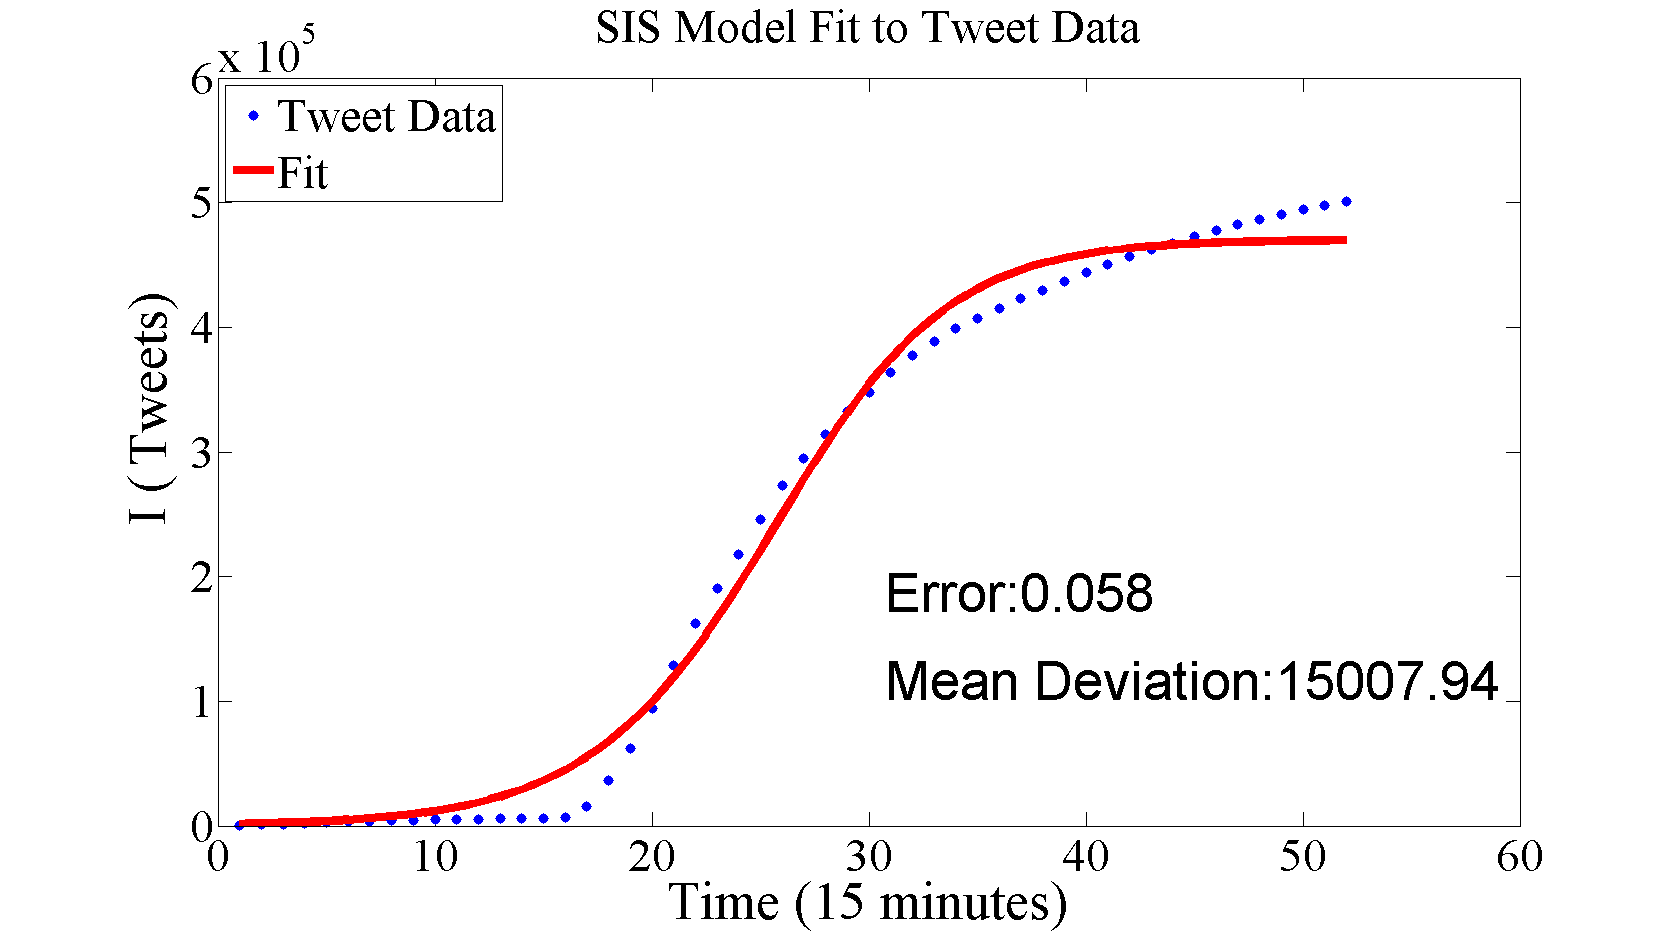
\includegraphics[width=2in,height=1.5in] {pictures/Boston_SIS.png}
  \label{fig:Boston_bombing_sis}
 }
 \subfigure[SEIZ]{
   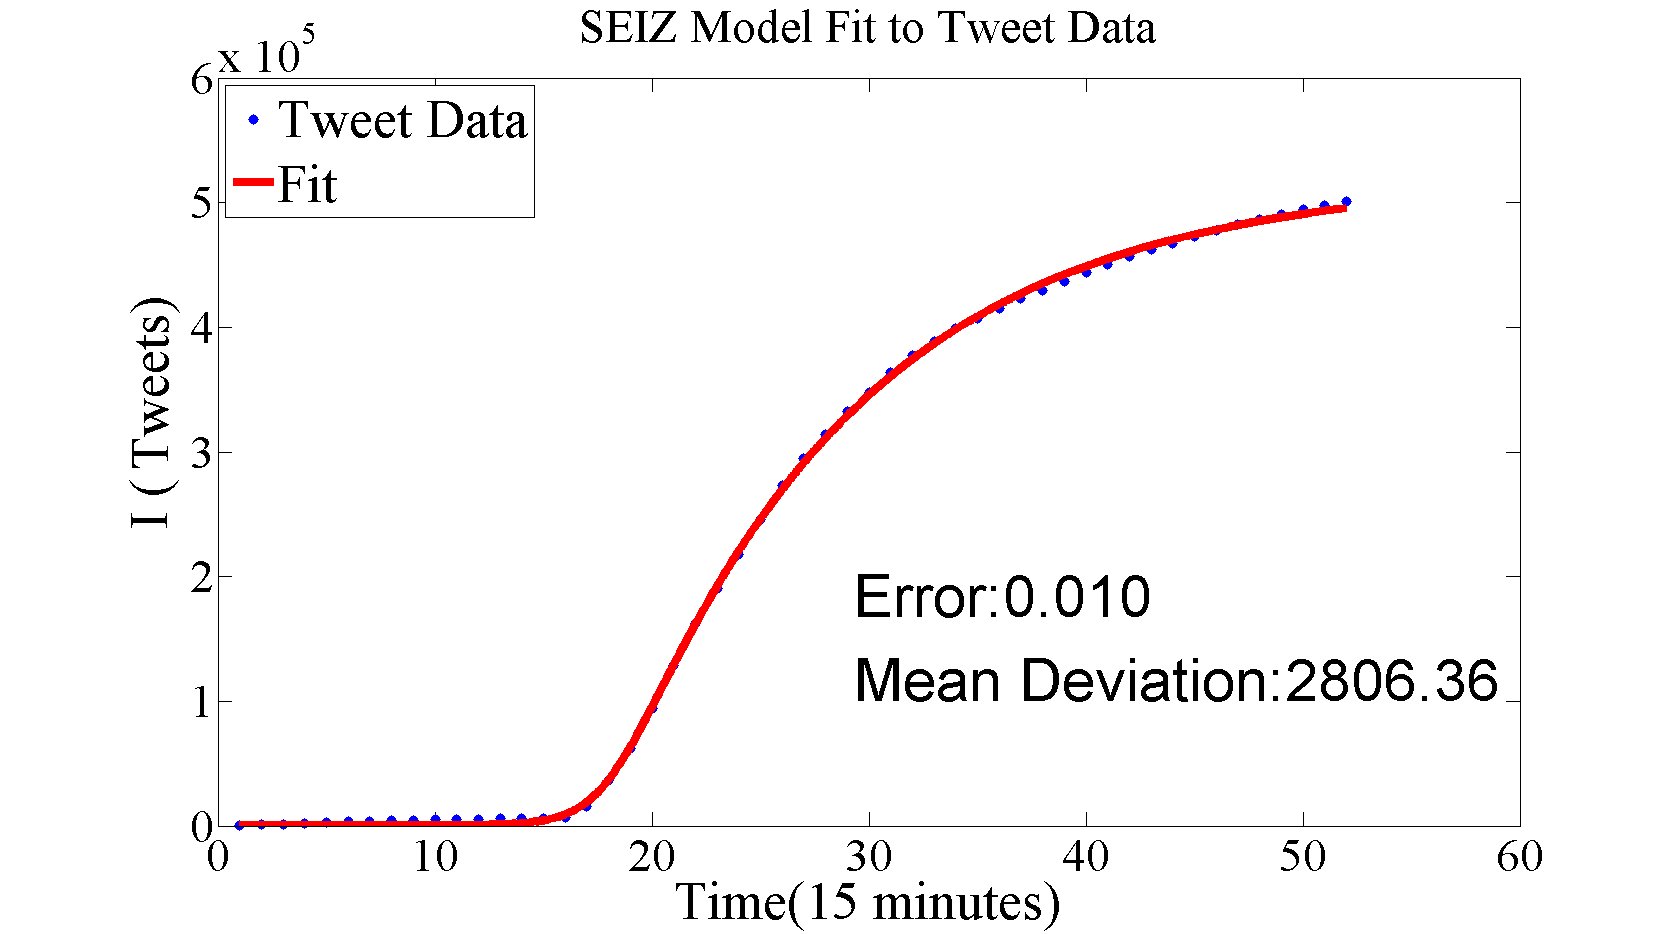
\includegraphics[width=2in,height=1.5in] {pictures/Boston_SEIZ.png}
  \label{fig:Boston_bombing_seiz}
 }
\vspace{-1em}
\caption{Best fit modeling for Boston news.}
\label{fig:Boston_bombing}
\end{figure}


\begin{figure}[t]
\centering
\subfigure[SIS]{
   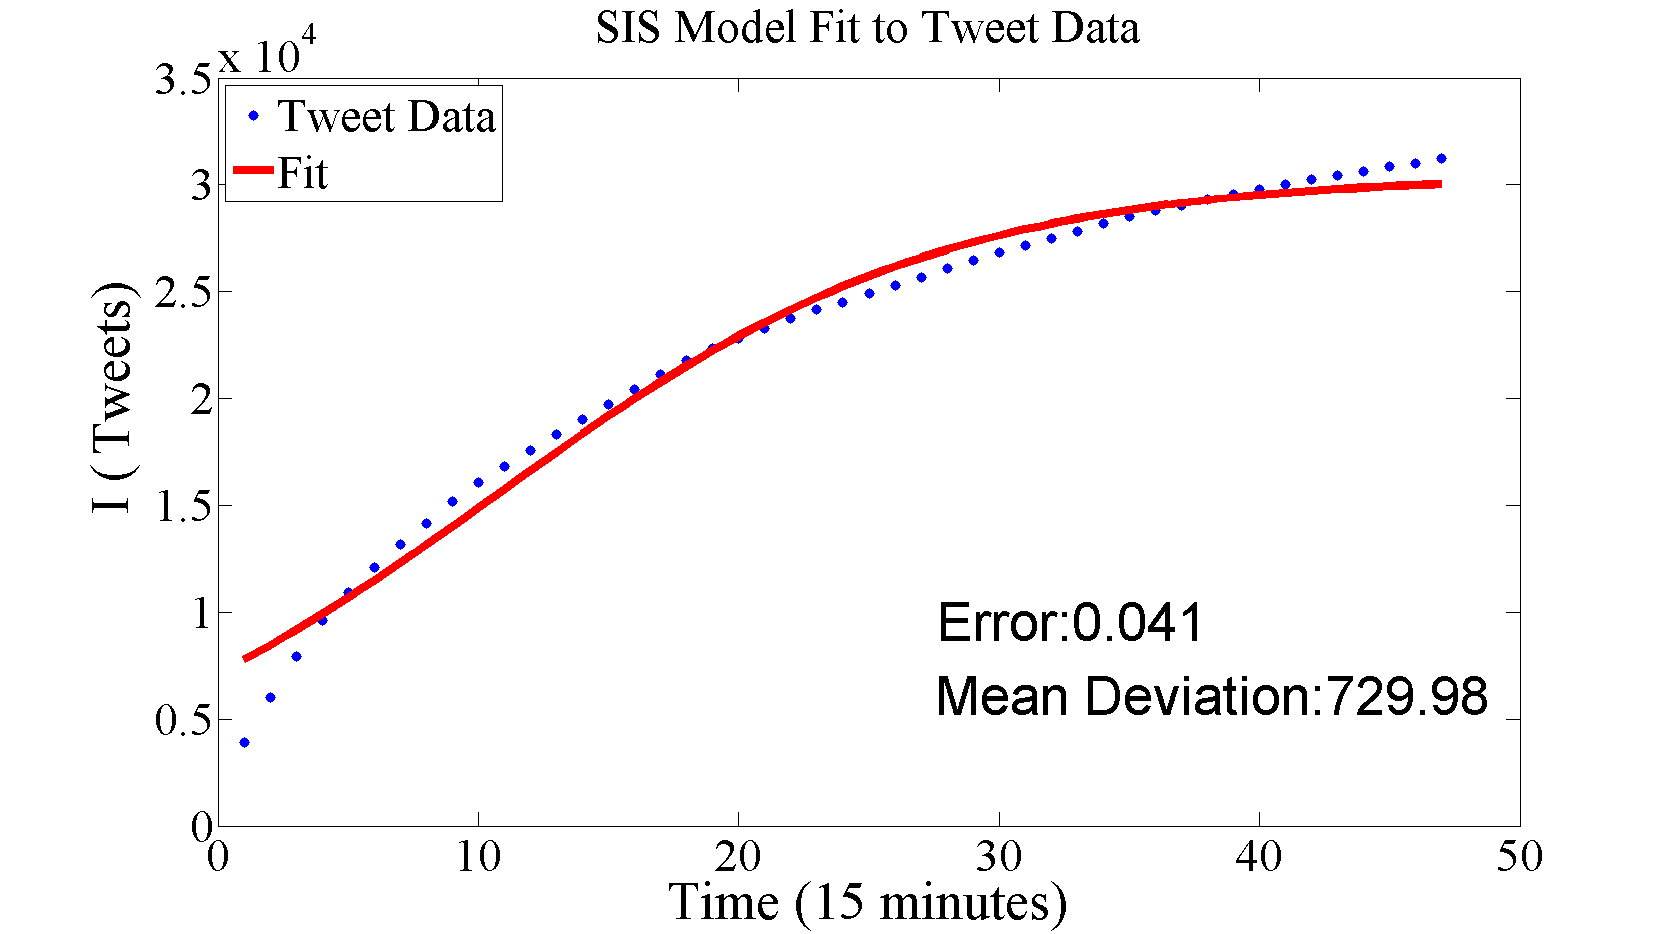
\includegraphics[width=2in,height=1.5in] {pictures/Pope_SIS.png}
  \label{fig:Benedict_sis}
 }
  \subfigure[SEIZ]{
   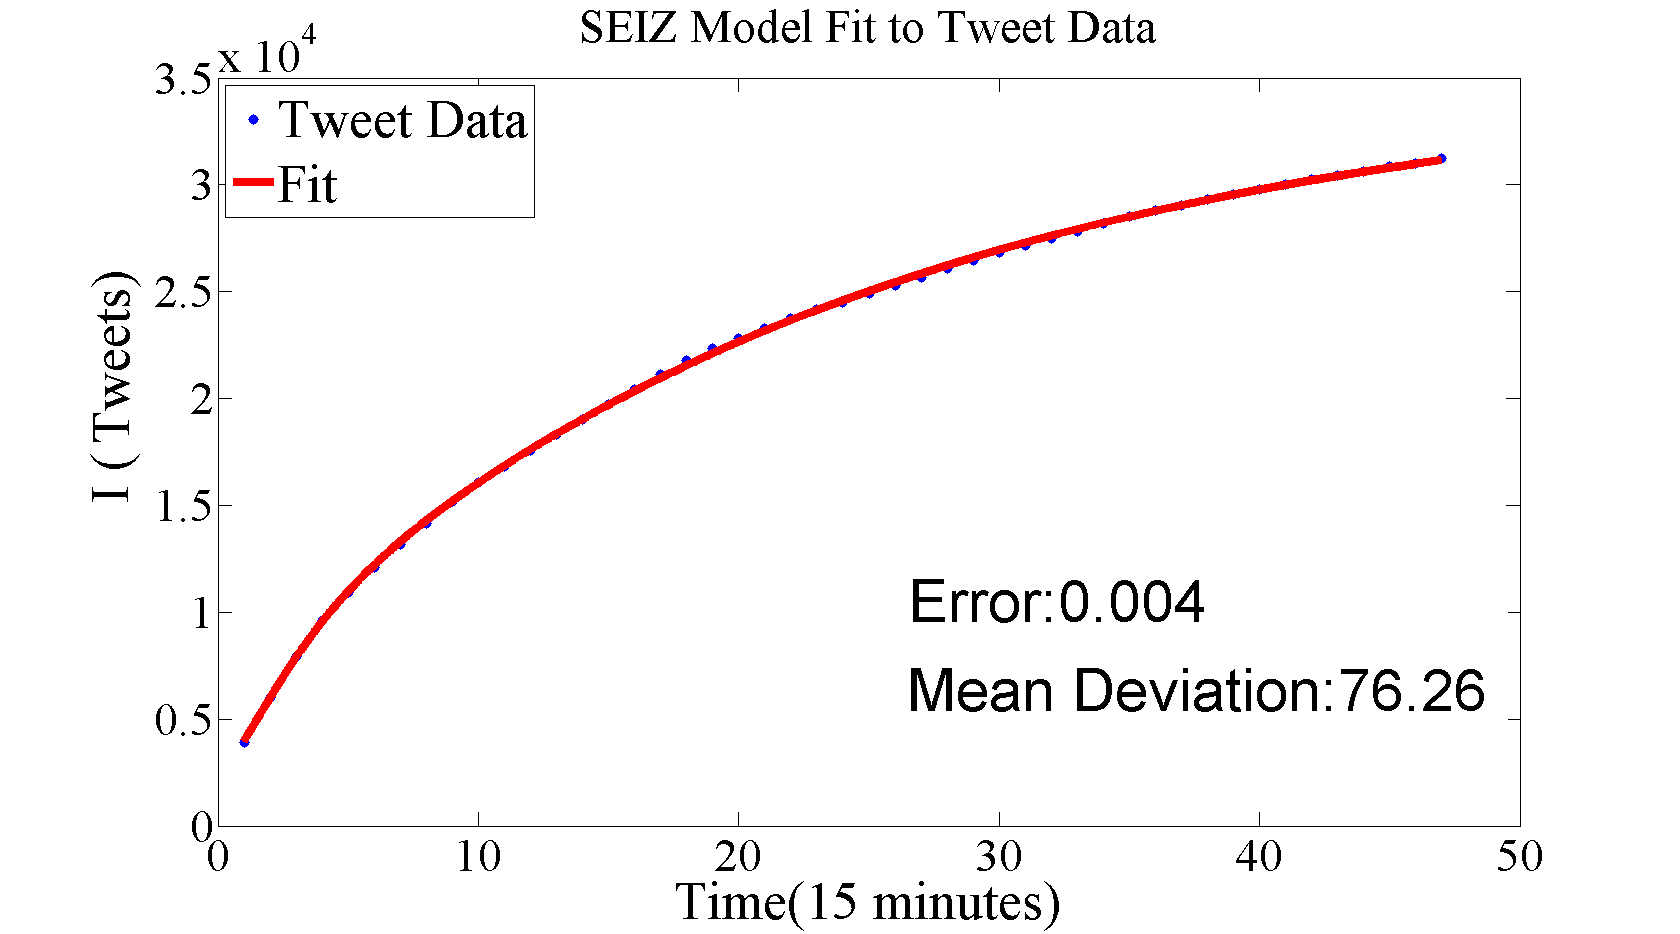
\includegraphics[width=2in,height=1.5in] {pictures/Pope_SEIZ.png}
  \label{fig:Benedict_seiz}
 }
\vspace{-1em}
\caption{Best fit modeling for Pope news.
\label{fig:Benedict}
}
\end{figure}


\begin{figure}[t]
\centering
\subfigure[SIS]{
   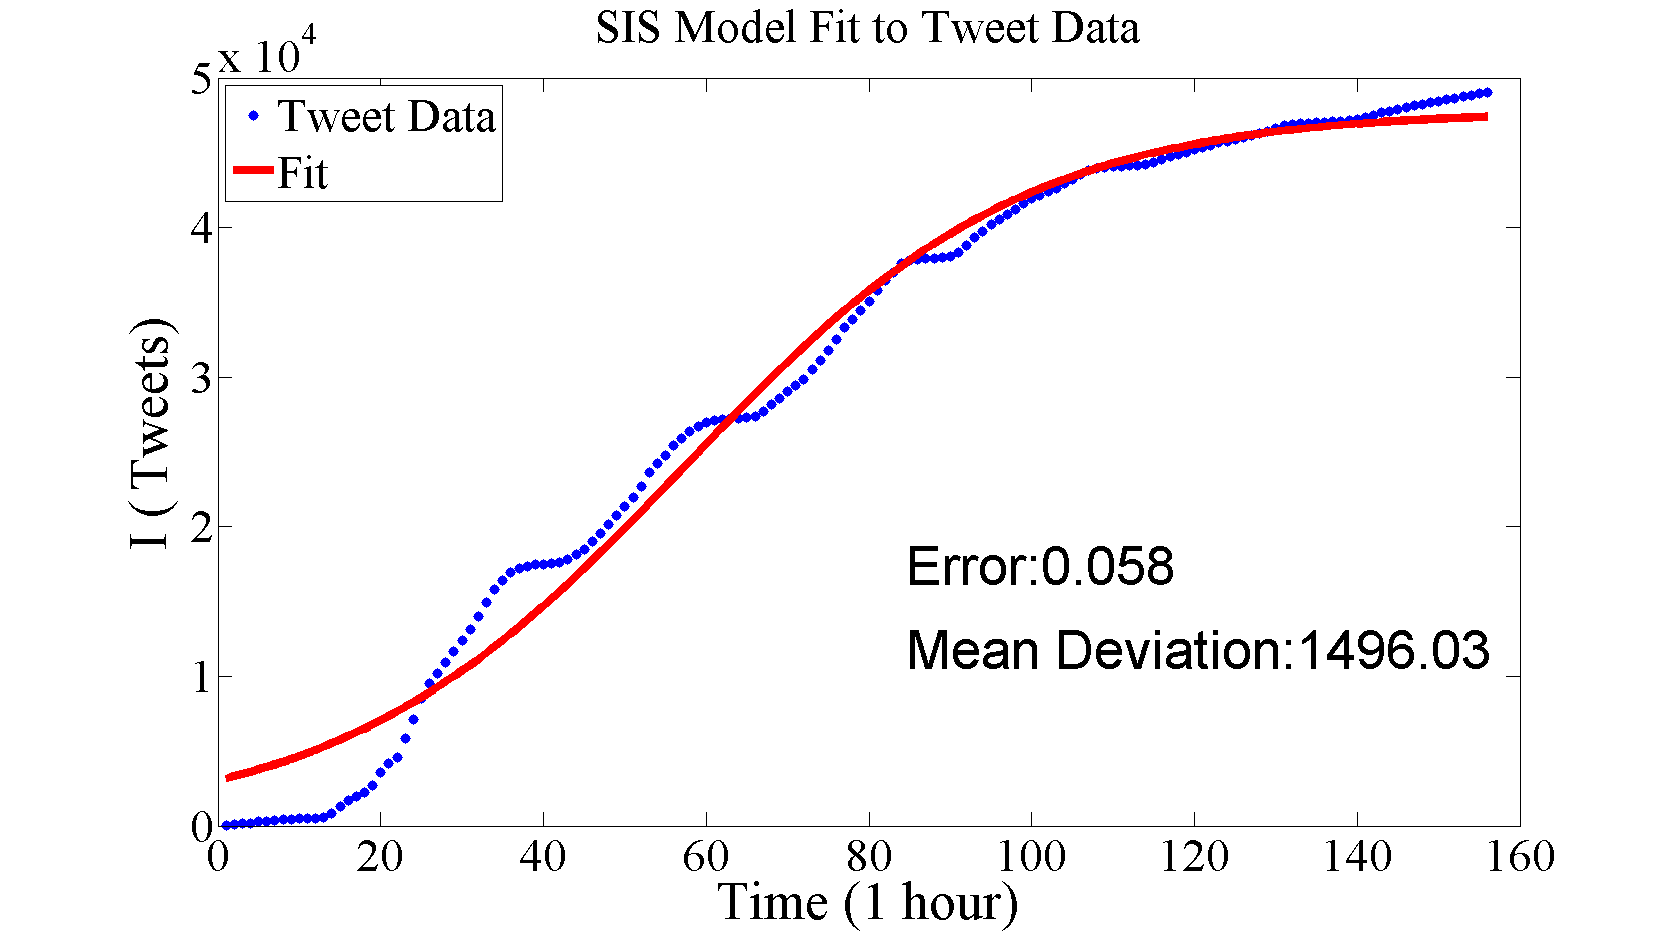
\includegraphics[width=2in,height=1.5in] {pictures/Amuay_SIS.png}
  \label{fig:Gas_explosion_sis}
 }
  \subfigure[SEIZ]{
   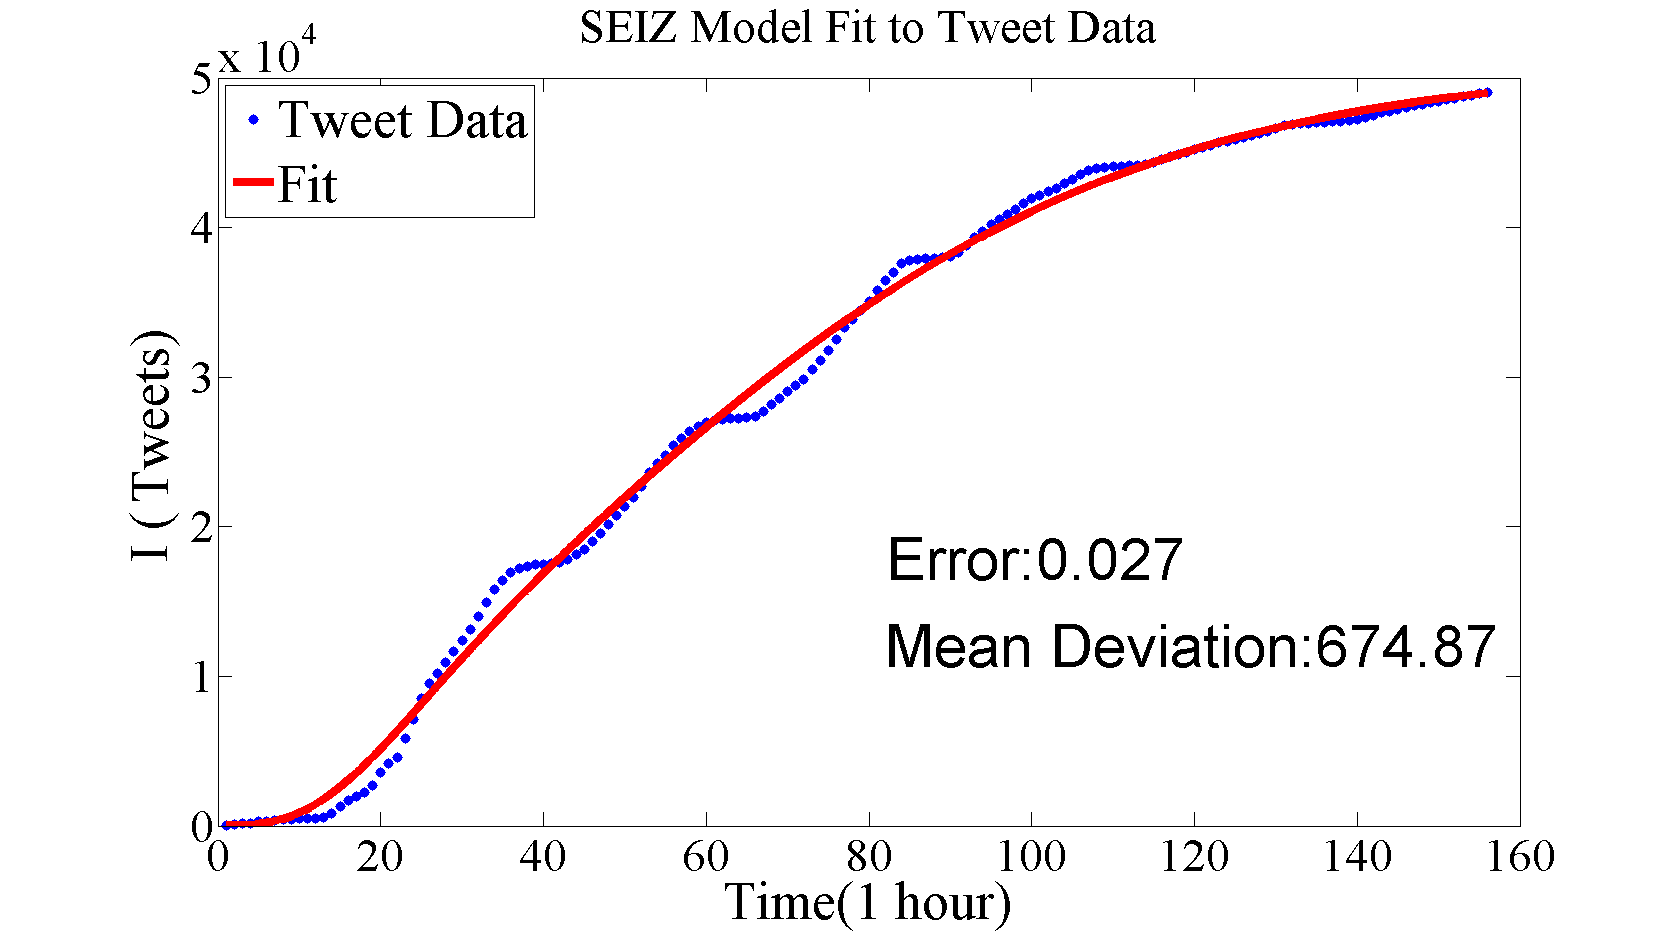
\includegraphics[width=2in,height=1.5in] {pictures/Amuay_SEIZ.png}
  \label{fig:Gas_explosion_seiz}
 }
\vspace{-1em}
\caption{Best fit modeling for Amuay news.}
\label{fig:Gas_explosion}
\end{figure}



\begin{figure}[t]
\centering
\subfigure[SIS]{
   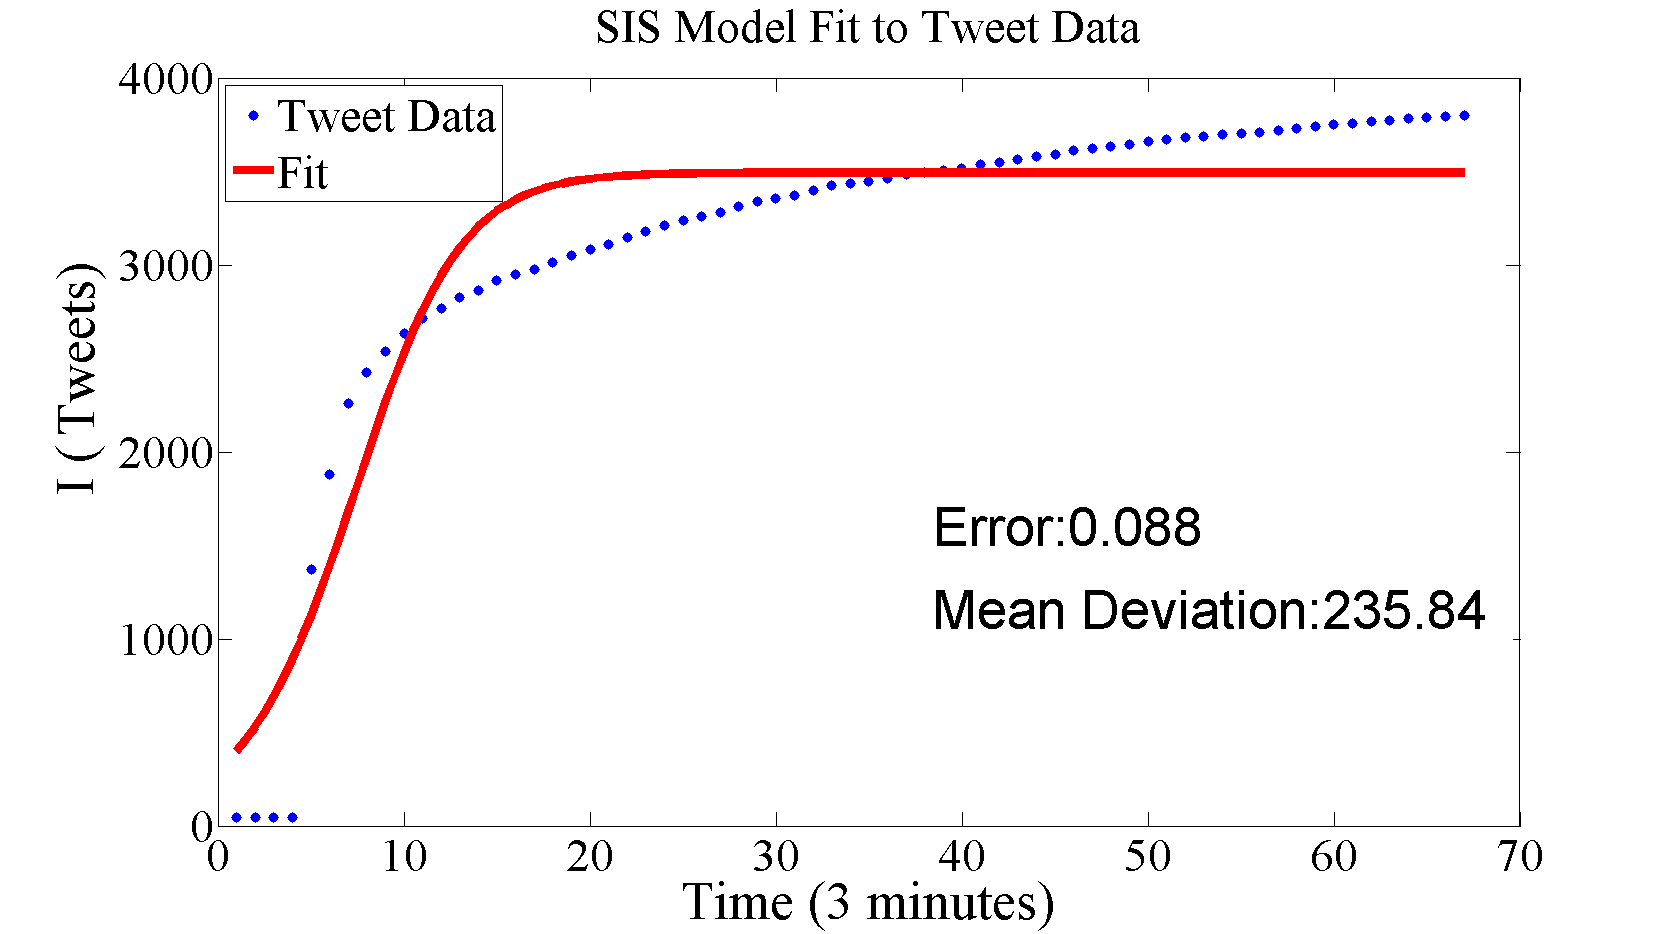
\includegraphics[width=2in,height=1.5in] {pictures/Michelle_SIS.png}
  \label{fig:Michelle_sis}
 }
  \subfigure[SEIZ]{
   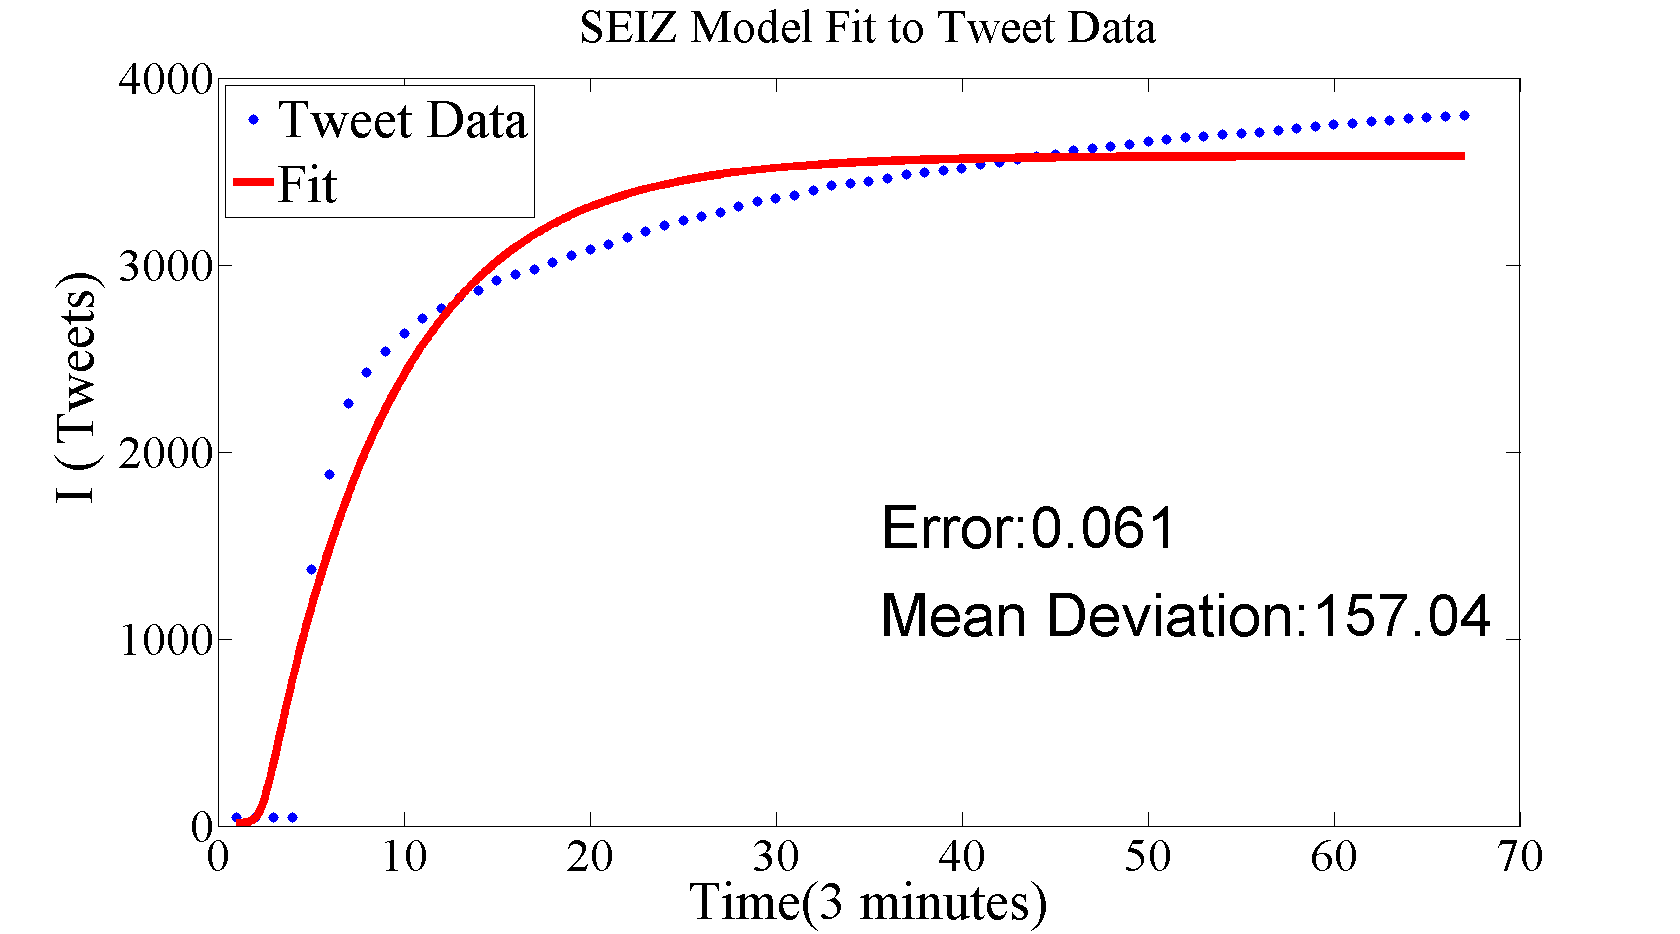
\includegraphics[width=2in,height=1.5in] {pictures/Michelle_SEIZ.png}
  \label{fig:Michelle_seiz}
 }
\vspace{-1.08em}
\caption{Best fit modeling for Michelle news.}
\label{fig:Michelle}
\end{figure}


\begin{figure}[ht]
\centering
\subfigure[SIS]{
   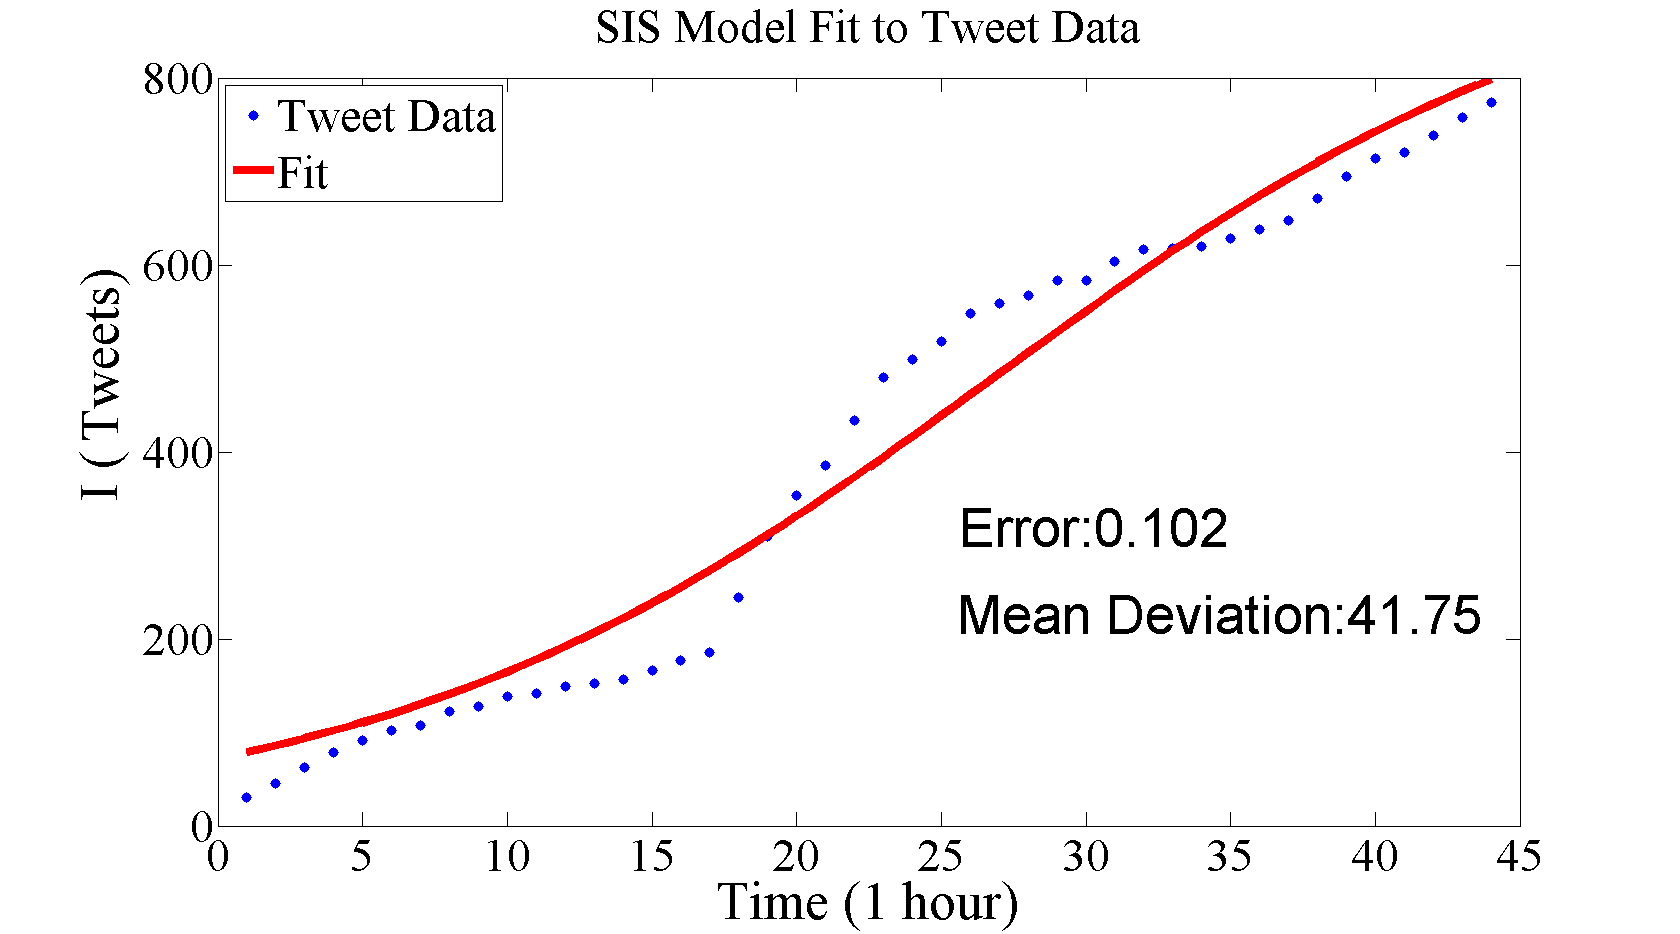
\includegraphics[width=2in,height=1.5in] {pictures/Obama_SIS.png}
  \label{fig:Obama_sis}
 }
 \subfigure[SEIZ]{
   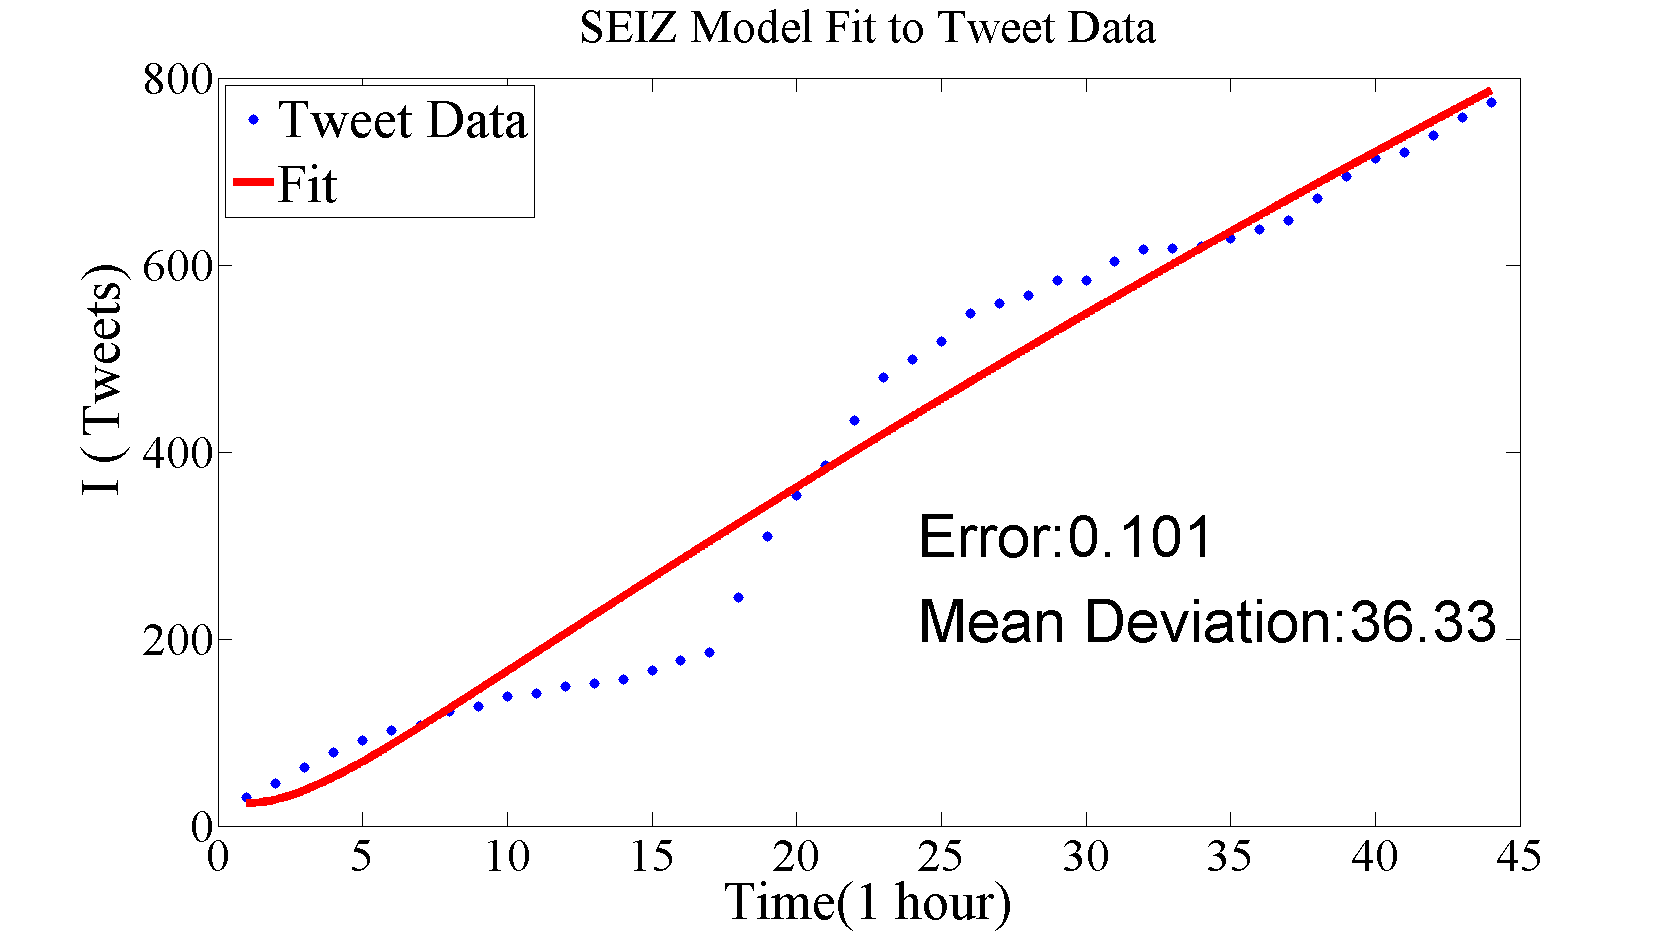
\includegraphics[width=2in,height=1.5in] {pictures/Obama_SEIZ.png}
   \label{fig:Obama_seiz}
 }
\vspace{-1em}
\caption{Best fit modeling for Obama news.}
\label{fig:Obama}
\end{figure}


\begin{figure}[ht]
\centering
\subfigure[SIS]{
   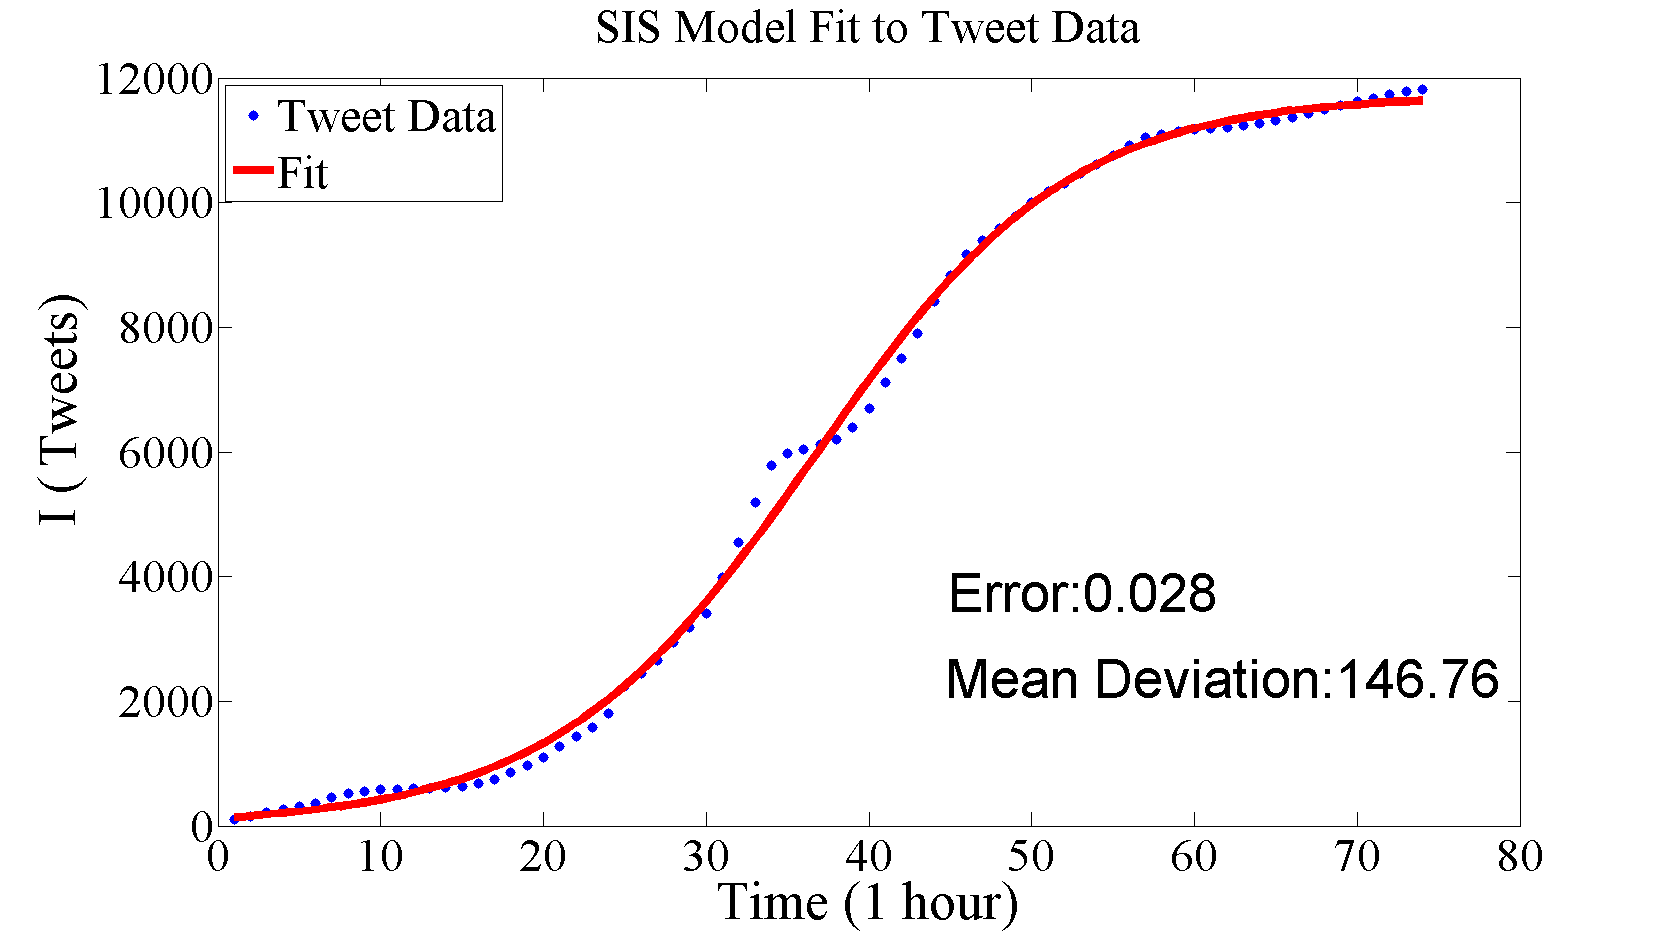
\includegraphics[width=2in,height=1.5in] {pictures/Doom_SIS.png}
   \label{fig:Doomsday_sis}
 }
   \subfigure[SEIZ]{
   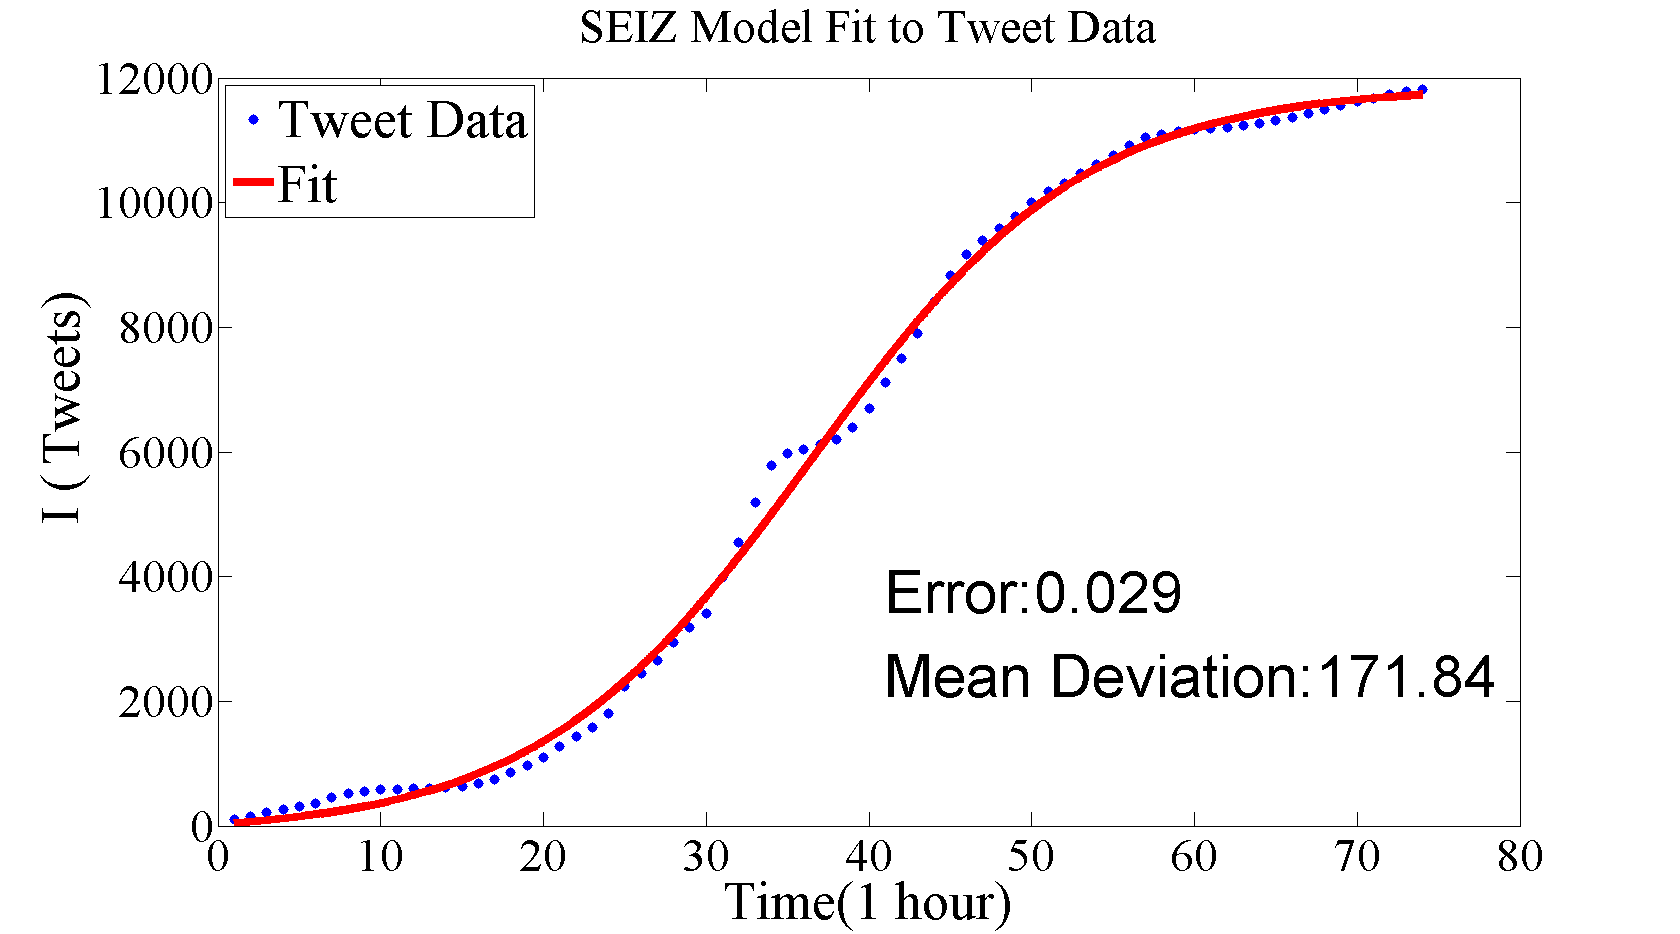
\includegraphics[width=2in,height=1.5in] {pictures/Doom_SEIZ.png}
   \label{fig:Doomsday_seiz}
 }
\vspace{-1em}
\caption{Best fit modeling for Doomsday rumor.}
\label{fig:Doomsday}
\end{figure}





\begin{table*}[t]
\tiny
\caption{Fitting error of SIS and SEIZ models}
\vspace{0.5em}
\centering
\begin{tabular}{| p{0.8cm}| p{1.2cm}| p{1cm} | p{1cm}| p{1.2cm} | p{1.3cm} | p{1.5cm} | p{1.2cm} | p{1.2cm}| p{1.3cm}| }
\hline
&\textbf{Boston}& \textbf{Pope} & \textbf{Amuay} & \textbf{Michelle} & \textbf{Obama} &\textbf{Doomsday} &\textbf{Castro}& \textbf{Riot}& \textbf{Average}   \\ [1ex]
\hline
\textbf{$SIS$} & 0.058 &0.041 & 0.058 & 0.088 & 0.102 & 0.028 & 0.082 & 0.088 & 0.068\\[1ex]
\hline
\textbf{$SEIZ$} & 0.010 & 0.004 &0.027 & 0.061 &0.101 & 0.029 & 0.073 & 0.093 & 0.050 \\[1ex]
\hline
\end{tabular}
\label{table:error} % is used to refer this table in the text
\end{table*}


Another constraint is the inability to quantify the total population size. This value appears to simply be the total number of Twitter accounts; however the value that we truly want is the number of individuals {\bf who could be exposed to the news or rumor topic}. This value shows to be very different from the total number of Twitter accounts. Consider the $\sim$175 million (M) registered Twitter accounts. Of these, (i) $\sim$90 million have no followers, and (ii) $\sim$56 million follow no one\footnote{http://www.businessinsider.com/chart-of-the-day-how-many-users-does-twitter-really-have-2011-3}. To further complicate the matter, there exists an abundance of
``fake'' Twitter accounts, which are never used by any real person. They are simply sold to users wishing to enhance their perceived popularity. Coupling these facts with sporadic Twitter usage due to night-time inactivity and user ``unplugging", it is clear that establishing a reliable estimate of users who could receive a tweet is quite difficult.

Synthesizing all of these factors, we assume the following in our SEIZ model implementation:
 %1) We do not have reliable population specifics:   		we do not know $N$, total population size; we do not know $S(t_0), E(t_0), I(t_0), $ or $Z(t_0)$,  the initial values of each population compartment. 2) Infected individuals ($I$) submit a tweet. 3) Skeptics ($Z$) have been exposed to story, but do not tweet. 4) Vital dynamics do not contribute to the overall population size. Thus, $N$ is a constant.

\begin{enumerate}
\item   We do not have reliable population specifics.
	\begin{enumerate}
    		\item We do not know $N$, total population size.
    		\item We do not know $S(t_0), E(t_0), I(t_0), $ or $Z(t_0)$,  the initial values of each population compartment.
  	\end{enumerate}
\item  {\bf Infected} individuals ($I$) submit a tweet.

\item  {\bf Skeptics} ($Z$) have been exposed to story, but do not tweet.

\item  Vital dynamics do not contribute to the overall population size. Thus, $N$ is a constant.
\end{enumerate}


The implication of these assumptions is that total population size N and initial population sizes for each compartment $S(t_0), E(t_0), I(t_0), $ and $Z(t_0)$ are viewed as unknowns. They are therefore treated as parameters in the parameter fit routine, and fit along with the other model parameters \cite{powerofgoodidea:2006}.

\subsection{Parameter Identification}

For each of the population models (SIS and SEIZ), represented by equation sets~\ref{eq:sis} and~\ref{eq:seiz}, we performed a nonlinear least squares fit of the model to Twitter data. As shown in Figure~\ref{fig:implementation_flow}, each step of this fitting process involved selecting a set of parameter values (rate constants and probabilities in equations \ref{eq:sis} and \ref{eq:seiz}, and initial compartment sizes), and numerically solving the system of ODEs with these parameter values. The set of parameter values that minimized $|I(t)-tweets(t)|$ was identified as the optimal parameter set.

The experimental implementation was done in Matlab. The {\bf lsqnonlin} function performed the least squares fit. The ODE systems were solved with a forward Euler function that we developed. This algorithm was selected due to its computational efficiency, and used a time-step of no more than 0.05. This threshold demonstrated to be numerically stable; in several instances we compared the forward Euler solution to those generated by Matlab's ode45 ($5^{th}$-order Explicit Runge-Kutta with embedded $4^{th}$-order error control), and observed nearly identical solutions.



\begin{figure}[t]
\centering
\subfigure[SIS]{
   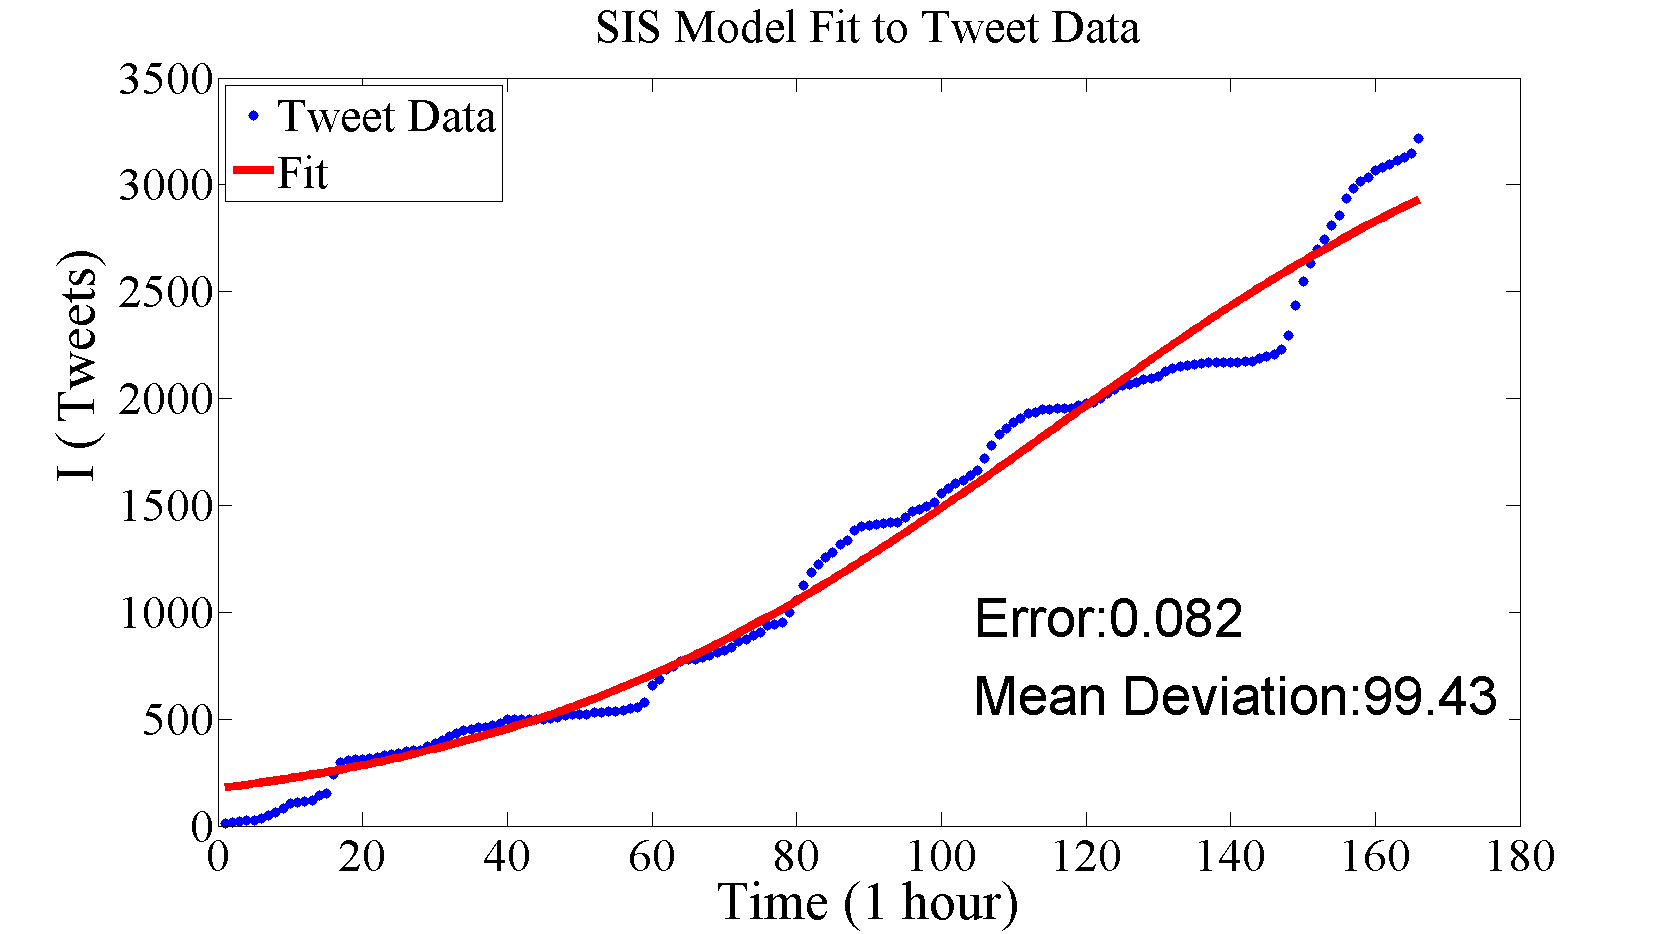
\includegraphics[width=2in,height=1.5in] {pictures/Castro_SIS.png}
   \label{fig:Castro_sis}
 }
  \subfigure[SEIZ]{
   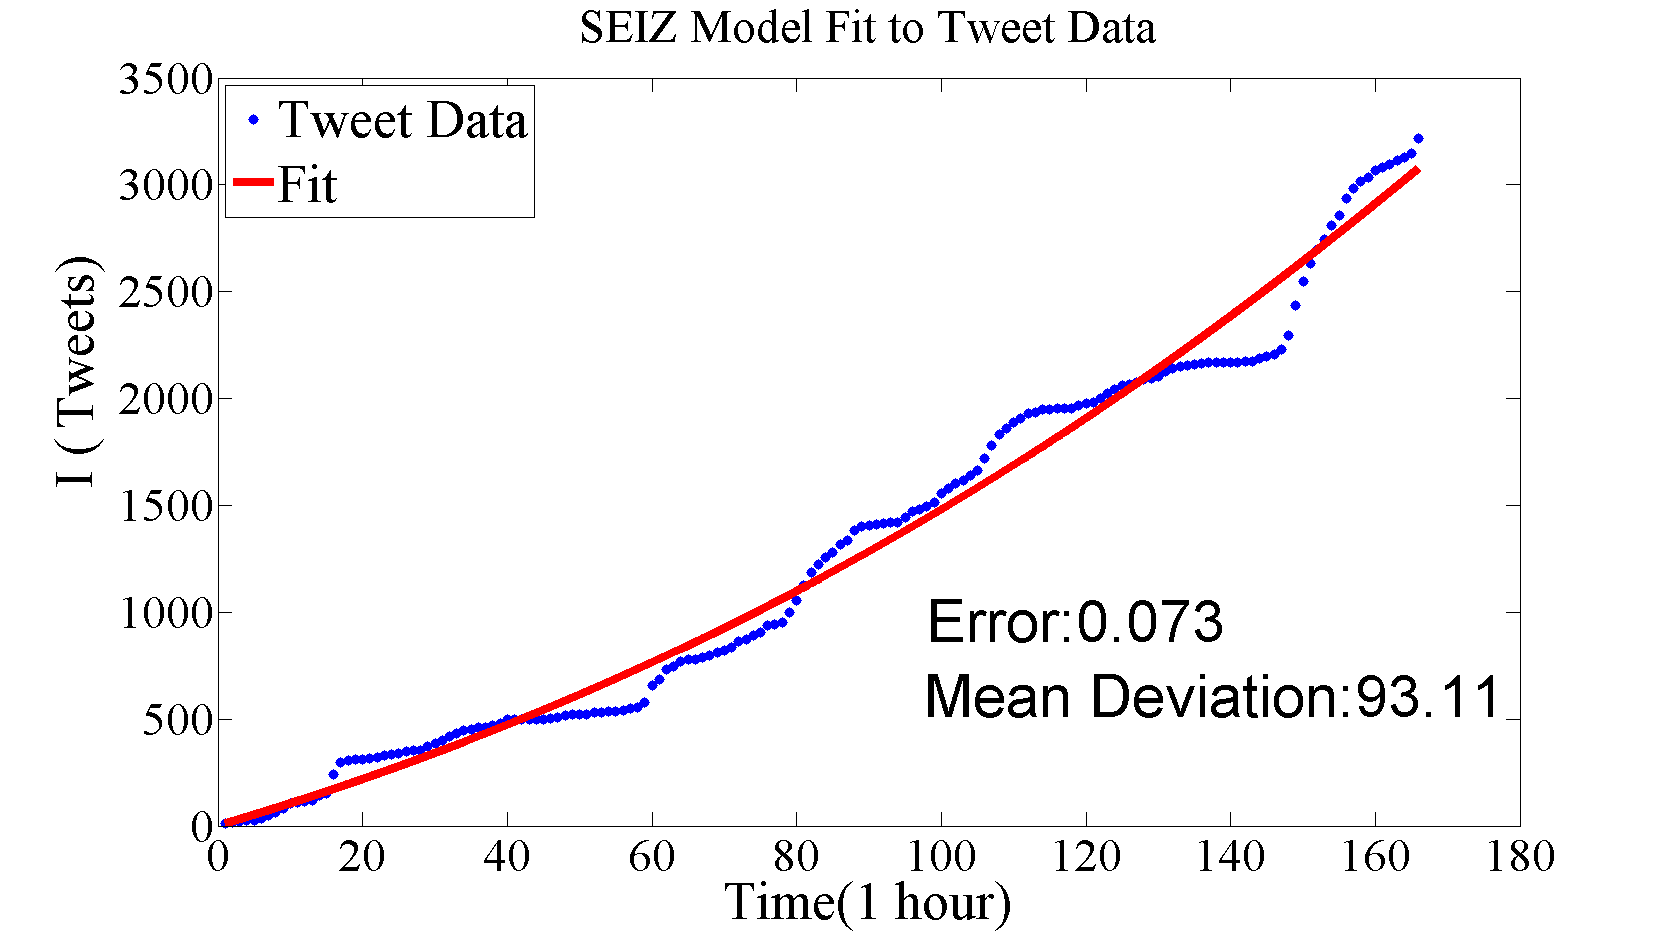
\includegraphics[width=2in,height=1.5in] {pictures/Castro_SEIZ.png}
   \label{fig:Castro_seiz}
 }
\vspace{-1.2em}
\caption{Best fit modeling for Castro rumor.}
\label{fig:Castro}
\end{figure}


\begin{figure}[t]
\centering
\subfigure[SIS]{
   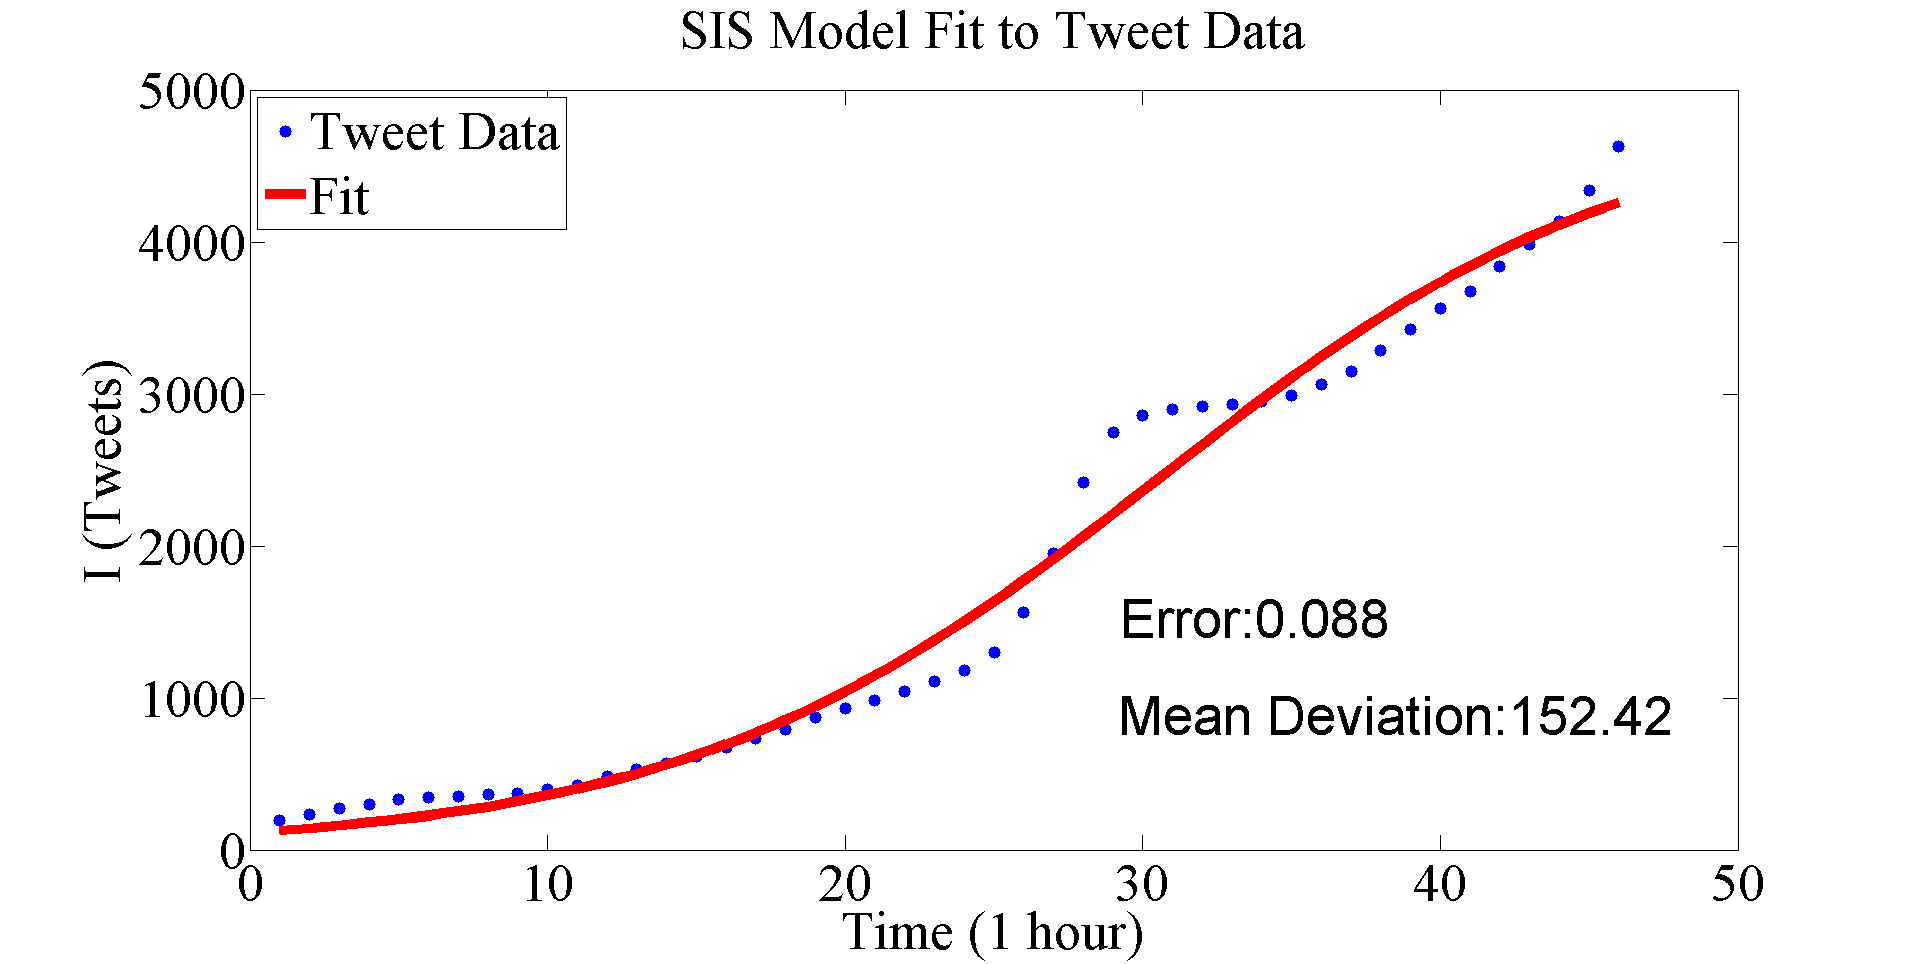
\includegraphics[width=2in,height=1.5in] {pictures/Riot_SIS.png}
  \label{fig:Mexico_riot_sis}
 }
  \subfigure[SEIZ]{
   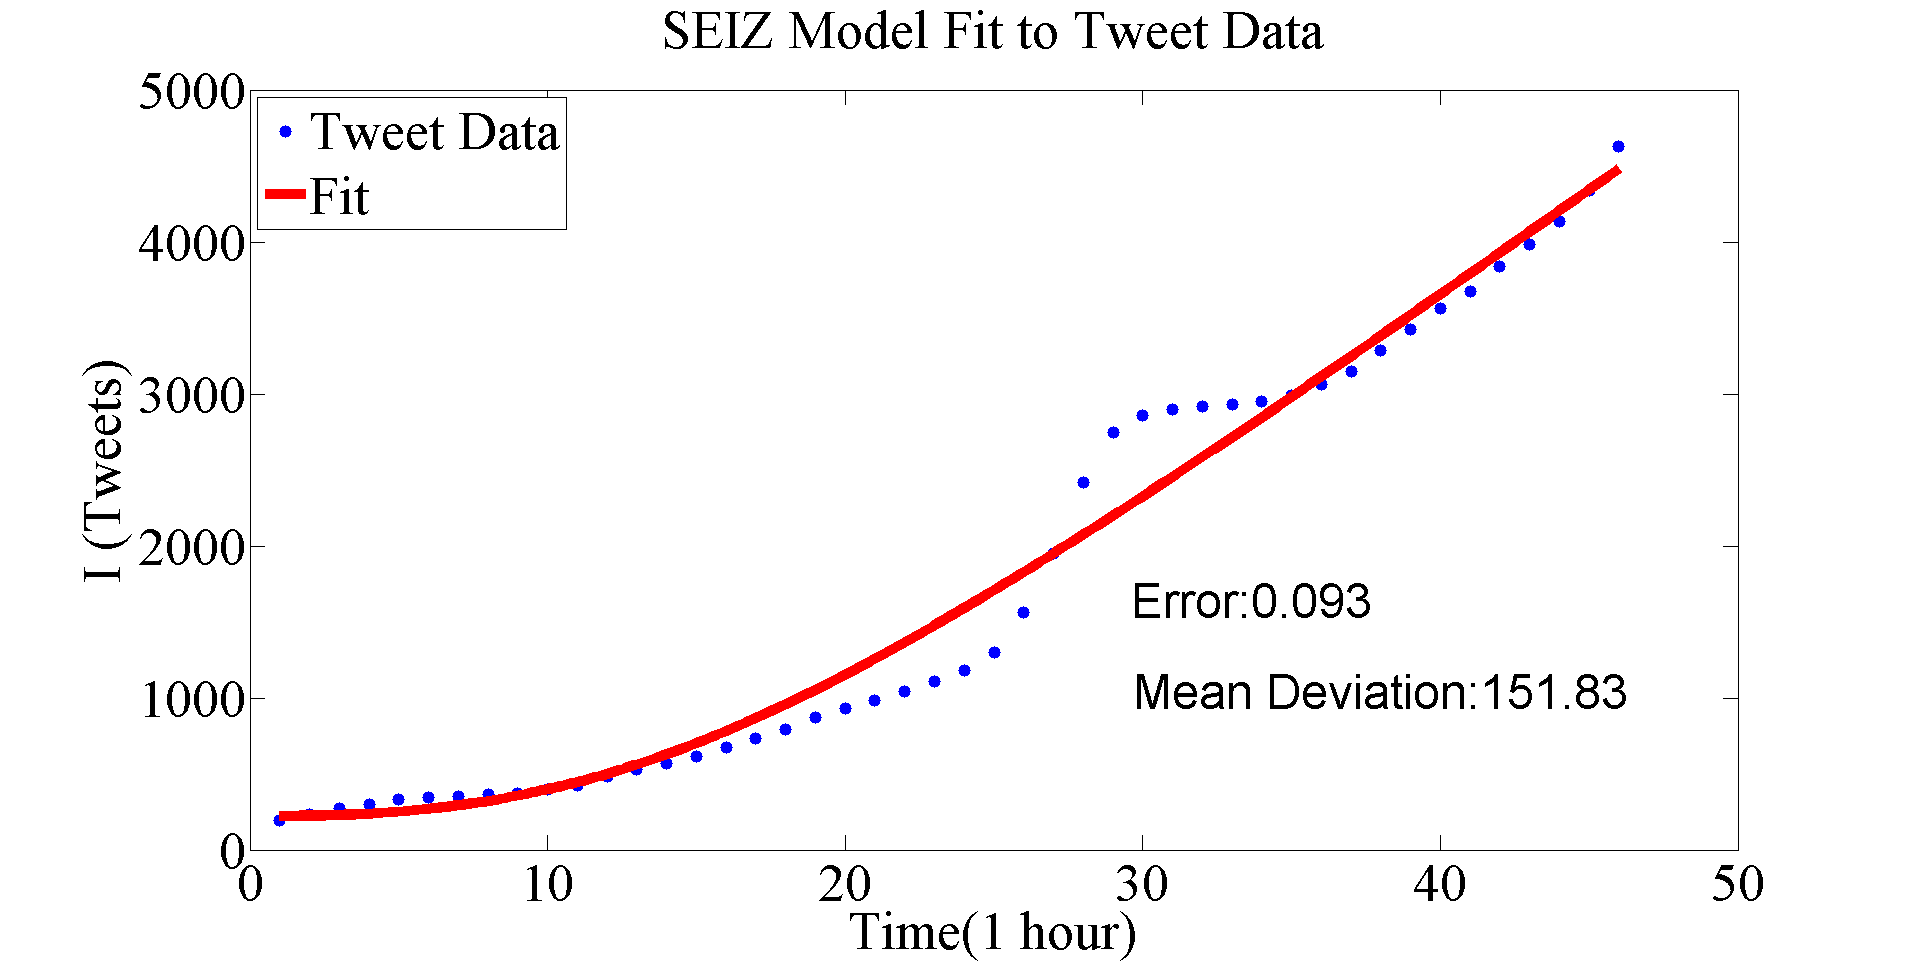
\includegraphics[width=2in,height=1.5in] {pictures/Riot_SEIZ.png}
  \label{fig:Mexico_riot_seiz}
 }
\vspace{-1.2em}
\caption{Best fit modeling for Riot news.}
\label{fig:Mexico_riot}
\end{figure}

